% Experiments
\chapter{Πειράματα}
\label{chapter:experiments}
Από τα πιο σημαντικά βήματα στη κατασκευή μεγάλων συστημάτων, όπως αυτό που αναπτύχθηκε στα πλαίσια της παρούσας εργασίας, είναι η επιλογή των παραμέτρων του συστήματος. Σε αυτό το κεφάλαιο παρουσιάζονται, τα βήματα που ακολουθήθηκαν για τις επιλογές των μοντέλων μηχανικής μάθησης του \emph{Retriever} και του \emph{Reader}, για την επιλογή των εσωτερικών τους παραμέτρων αλλά και πως πραγματοποιήθηκε η αξιολόγηση των μοντέλων ταξινόμησης. Κάθε κόμβος του συστήματος αξιολογήθηκε χωριστά από τον άλλο και στο τέλος γίνεται και αξιολόγηση του συνολικού συστήματος. Επίσης, σχολιάζονται οι μετρικές που χρησιμοποιήθηκαν αλλά και τα σύνολα των δεδομένων αξιολόγησης.

\section{Σύνολο Δεδομένων Αξιολόγησης}
\label{sec:eval-dataset}
Εξαιτίας της έλλειψης συνόλων δεδομένων, πέρα από την ανάπτυξη μοντέλων μηχανικής μάθησης, καθίσταται δύσκολη και η αξιολόγηση των ελληνικών συστημάτων ειδικά αυτά που αφορούν συστήματα ερώτησης-απάντησης. Το \emph{XQuAD} \cite{xquad} είναι ένα διαγλωσσικό σύνολο δεδομένων ερώτησης απάντησης που αποτελείται από $240$ παραγράφους και $1190$ ερωτήσεις και είναι επαγγελματικά μεταφρασμένο για διάφορες γλώσσες ανάμεσα στις οποίες είναι και τα ελληνικά.

Για την αξιολόγηση των μοντέλων ταξινόμησης χρησιμοποιήθηκε μέρος του συνόλου των άρθρων που αποκτήθηκαν με τη μέθοδο που περιγράφεται στο \autoref{sec:soup}. Τα άρθρα λήφθηκαν από τρεις δημοφιλής ιστοσελίδες, μία για αθλητικές ειδήσεις, μία για πολιτικές ειδήσεις και μία για ειδήσεις τεχνολογίας, ταινιών και \emph{gaming}. Τα άρθρα της κατηγορίας άλλο (\emph{other}) λήφθηκαν με παρόμοιο τρόπο από το σύνολο δεδομένων της εφημερίδας Μακεδονία\footnote{\url{https://www.greek-language.gr/greekLang/modern_greek/tools/corpora/makedonia/content.html}}, από κατηγορίες που δεν επικάλυπταν τις παραπάνω. Για κάθε ένα από τα άρθρα που αποθηκεύονται στη βάση δεδομένων, εκτός από το περιεχόμενο αποθηκεύονται επίσης το όνομα του αρχείου, ο τίτλος του άρθρου, το \emph{ulr} της ιστοσελίδας από την οποία προήλθε το άρθρο, η κατηγορία του και η ημερομηνία έκδοσης του. Το σύνολο των ληφθέντων άρθρων και ένα παράδειγμα ενός άρθρου αποθηκευμένου στη βάση φαίνονται στους πίνακες \ref{tab:dataset} και \ref{tab:dataset-sample} αντίστοιχα.

\begin{table}[htb]
    \captionsetup{justification=centering}
    \begin{center}
        \caption{Σύνολο δεδομένων κάθε μίας από τις κατηγορίες των άρθρων}
        \begin{tabular}{ | c | c |}
            \hline
            \rowcolor{Gray}
            Κατηγορία & Αριθμός άρθρων\\
            αθλητικά & $5468$\\
            πολιτική & $1483$\\
            τεχνολογία & $1329$\\
            \emph{gaming} & $1273$\\
            ταινίες &  $1222$\\
            άλλο & $1427$\\
            \hline
            \hline
            \emph{Σύνολο} & $12202$\\
            \hline
        \end{tabular}
        \label{tab:dataset}
    \end{center}
\end{table}

\begin{table}[htb]
    \captionsetup{justification=centering}
    \begin{center}
        % \begin{tabular}{ |p{\columncolor[gray]{2.5cm}}|p{2cm}|p{2cm}|p{2cm}|p{2cm}|p{2.5cm}|}
        %     % \hline
        %     % \rowcolor{Gray}
        %     Περιεχόμενο & Όνομα αρχείου & Τίτλος & Url & Κατηγορία & Ημερομηνία έκδοσης\\
        %     Μαζί με το Mac Studio παρουσιάστηκε και το Studio Display, μία οθόνη με σώμα αλουμινίου ... & apple studio display .json & Studio Display: Η οθόνη της Apple έχει ένα Α13 Bionic και κάμερα iPhone & https:// url.com/ article0 & \emph{tech} & 2022-04-30\\
        %     \hline
        % \end{tabular}
        \caption{Παράδειγμα αποθηκευμένου άρθρου στη βάση δεδομένων}
        \begin{tabular}{|>{\columncolor[gray]{0.8}}c|m{9cm}|}
        \hline
            Περιεχόμενο & Μαζί με το Mac Studio παρουσιάστηκε και το Studio Display, μία οθόνη με σώμα αλουμινίου ...\\\hline
            Όνομα αρχείου & apple\_studio\_display.json\\\hline
            Τίτλος & Studio Display: Η οθόνη της Apple έχει ένα Α13 Bionic και κάμερα iPhone\\\hline
            Url & https://url.com/article0\\\hline
            Κατηγορία & \emph{tech}\\\hline
            Ημερομηνία έκδοσης & 2022-04-30\\\hline
        \end{tabular}
        \label{tab:dataset-sample}
    \end{center}
\end{table}

\section{Μετρικές Αξιολόγησης Συστημάτων}
\label{sec:metrics}
\subsection{Αξιολόγηση μοντέλων ταξινόμησης}
Μια ταξινόμηση ορίζεται ως αληθώς θετική (\emph{True Positive - TP}) όταν όταν ταξινομείται σωστά στη θετική κλάση, ως ψευδώς αρνητική (\emph{False Negative - FN}) όταν ταξινομείται σε κλάση διαφορετική της θετικής, ενώ ανήκει στη θετική, ως ψευδώς θετική (\emph{False Positive - FP}) όταν ταξινομείται στη θετική κλάση ενώ δεν ανήκει σε αυτή και ως αληθώς αρνητική (True Negative - TN) όταν δεν ανήκει στη θετική κλάση και δεν ταξινομείται σε αυτή. Με βάση αυτούς τους ορισμούς προκύπτουν οι μετρικές οι οποίες αξιοποιήθηκαν για την αξιολόγηση των μοντέλων ταξινόμησης.

\begin{itemize}
    \item \emph{Accuracy}: περιγράφει τον αριθμό των σωστών προβλέψεων σε σχέση με το συνολικό αριθμό των προβλέψεων, \autoref{eq:accuracy}
    \item \emph{Precision}: είναι ένα μέτρο για το πόσες από τις θετικές προβλέψεις είναι σωστές, \autoref{eq:precision}
    \item \emph{Recall}: είναι ο λόγος του αριθμού των θετικών προβλέψεων που ταξινομήθηκαν σωστά προς των συνολικό αριθμό των θετικών, \autoref{eq:recall}
    \item $F_1$ σκορ\footnote{Στους πίνακες που ακολουθούν παρουσιάζονται και οι μετρικές \emph{macro avg} και \emph{weighted avg} οι οποίες αποτελούν τον απλό και ζυγισμένο μέσο όρο του $F_1 Score$. Στο ζυγισμένο μέσο όρο λαμβάνεται υπόψιν και το \emph{support} κάθε κλάσης.} ($F_1 score$): είναι ένας συνδυασμός των \emph{precision} και \emph{recall}, \autoref{eq:f1-score}
    \item Υποστηριξη (\emph{Support}): δείχνει τον αριθμό των δειγμάτων κάθε κλάσης
\end{itemize}

\begin{align}
    &accuracy& &=& &\frac{\mathbf{TP} + \mathbf{TN}}{\mathbf{TP} + \mathbf{TN} + \mathbf{FP} + \mathbf{FN}} \label{eq:accuracy}\\
    &precision& &=& &\frac{\mathbf{TP}}{\mathbf{TP} + \mathbf{FP}}
    \label{eq:precision}\\
    &recall& &=& &\frac{\mathbf{TP}}{\mathbf{TP} + \mathbf{FN}}
    \label{eq:recall}\\
    &F_1 score& &=& &2 \cdot \frac{\mathbf{precision} \cdot \mathbf{recall}}{\mathbf{precision}+\mathbf{recall}}
    \label{eq:f1-score}
\end{align}

Σε προβλήματα ταξινόμησης όπου οι κλάσεις είναι παραπάνω των δύο, όπως και στη παρούσα περίπτωση όπου το άρθρο μπορεί να ταξινομηθεί σε μία από έξι πιθανές κλάσεις, τότε οι μετρικές που παρουσιάστηκαν παραπάνω εξάγονται για κάθε κλάση ορίζοντας διαδοχικά τη μία κλάση ως θετική και τις άλλες ως αρνητική.

\subsection{Αξιολόγηση μοντέλων \emph{Reader}}

Για την αξιολόγηση των μοντέλων των \emph{Reader} χρησιμοποιήθηκαν δύο μετρικές η απόλυτη ταύτιση (\emph{Exact Match, EM}) και μία παραλλαγή του \emph{$F_1 Score$} προσαρμοσμένη για συστήματα κατανόησης φυσικής γλώσσας. Το \emph{EM}, όπως μαρτυρά και η ονομασία του, αναφέρεται στη πλήρη ταύτιση της εξόδου του μοντέλου με την πραγματική απάντηση. Πιο συγκεκριμένα, είναι ο λόγος των σωστά προβλεπόμενων απαντήσεων από το μοντέλο, προς τις συνολικές. Γίνεται εύκολα αντιληπτό πως αυτή είναι μία αρκετά αυστηρή αξιολόγηση του μοντέλου καθώς η πρόβλεψη αυτού μπορεί να είναι πολύ κοντά στην πραγματική απάντηση, αλλά να διαφέρει για παράδειγμα κατά μία λέξη. Για το λόγο αυτό χρησιμοποιείται το \emph{$F_1 Score$}.

Ο υπολογισμός του \emph{$F_1 Score$} φαίνεται στην \autoref{eq:f1-score} όπου:
\begin{itemize}
    \item \textbf{\emph{precision}}: ο λόγος των κοινών λέξεων της προβλεπόμενης απάντησης με τη πραγματική, προς τον συνολικό αριθμό των λέξεων στην προβλεπόμενη απάντηση
    \item \textbf{\emph{recall}}: ο λόγος των κοινών λέξεων της προβλεπόμενης απάντησης με τη πραγματική, προς τον συνολικό αριθμό των λέξεων στην σωστή απάντηση
\end{itemize}

\section{\emph{Classification}}
\label{sec:classification_exp}
Για την ταξινόμηση των άρθρων μελετήθηκαν ένα \emph{MLP} και μία \emph{fine-tuned} έκδοση του \emph{greek-bert}, όπως αναφέρθηκε στο \autoref{sec:classification}. Από τα αποτελέσματα που παρουσιάζονται στους πίνακες \ref{tab:classification-mlp} και \ref{tab:classification-bert}, παρατηρείται ότι και τα δύο μοντέλα έχουν αρκετά καλά αποτελέσματα για όλες τις κλάσεις ταξινόμησης. Παρατηρήθηκε ωστόσο ότι το \emph{fine-tuning} του \emph{greek bert} χρειάζεται αρκετά περισσότερο χρόνο για την εκπαίδευση του σε σχέση με το απλό \emph{MLP} που σχεδιάστηκε. Παρόλα αυτά, το τελικό μοντέλο που επιλέγεται είναι αυτό του \emph{greek BERT} διότι η τεχνολογία του με τα \emph{transformers} επιτρέπει και τη νοηματική "κατανόηση" της εισόδου σε αντίθεση με το \emph{MLP} το οποίο χρησιμοποιεί τη μέθοδο \emph{TF-IDF}. Έτσι, αν για παράδειγμα ερχόταν ως είσοδος στο σύστημα μία ταινία η οποία δεν βρισκόταν στα δεδομένα εκπαίδευσης το \emph{BERT} θα ήταν πιο πιθανό να προβλέψει ότι το άρθρο αφορά ταινία από τα συμφραζόμενα της εισόδου, κάτι το οποίο σίγουρα δεν υποστηρίζεται από το \emph{MLP}.


\begin{table}[!htb]
    \captionsetup{justification=centering}
    \begin{center}
        \caption{Αποτελέσματα ταξινόμησης με το μοντέλο \emph{MLP}}
        \begin{tabular}{ | c | c | c | c | c |}
            \hline
            \rowcolor{Gray}
            Κατηγορία & \emph{precision} & \emph{recall} & \emph{$F_1$ Score} & \emph{support}\\
            αθλητικά & $98.9$ & $99.8$ & $99.4$ & $656$\\
            πολιτική & $98.9$ & $97.2$ & $98.0$ & $178$\\
            τεχνολογία & $94.6$ & $98.1$ & $96.3$ & $160$\\
            \emph{gaming} & $98.7$ & $96.1$ & $97.4$ & $153$\\
            ταινίες & $99.3$ & $98.6$ & $99.0$ & $147$\\
            άλλο & $97.0$ & $94.7$ & $95.9$ & $171$\\
            \hline
            \hline
            \multicolumn{1}{| c |}{\emph{macro avg}} & $97.9$ & $97.4$ & $97.7$ & $1465$\\
            \hline
            \multicolumn{1}{| c |}{\emph{weighted avg}} & $98.2$ & $98.2$ & $98.2$ & $1465$\\
            \hline
            \hline
            \multicolumn{1}{| c |}{\emph{Accuracy}} & \multicolumn{4}{| c |}{$98.2$}\\
            \hline
        \end{tabular}
        \label{tab:classification-mlp}
    \end{center}
\end{table}

\begin{table}[!htb]
    \captionsetup{justification=centering}
    \begin{center}
        \caption{Αποτελέσματα ταξινόμησης με το μοντέλο \emph{Greek Bert}}
        \begin{tabular}{ | c | c | c | c | c |}
            \hline
            \rowcolor{Gray}
            Κατηγορία & \emph{precision} & \emph{recall} & \emph{$F_1$ Score} & \emph{support}\\
            αθλητικά & $99.8$ & $99.4$ & $99.6$ & $656$\\
            πολιτική & $100.0$ & $100.0$ & $100.0$ & $178$\\
            τεχνολογία & $95.2$ & $98.8$ & $96.9$ & $160$\\
            \emph{gaming} & $98.0$ & $96.7$ & $97.4$ & $153$\\
            ταινίες & $98.6$ & $97.3$ & $97.9$ & $147$\\
            άλλο & $98.8$ & $99.4$ & $99.1$ & $171$\\
            \hline
            \hline
            \multicolumn{1}{| c |}{\emph{macro avg}} & $98.4$ & $98.6$ & $98.5$ & $1465$\\
            \hline
            \multicolumn{1}{| c |}{\emph{weighted avg}} & $98.9$ & $98.9$ & $98.9$ & $1465$\\
            \hline
            \hline
            \multicolumn{1}{| c |}{\emph{Accuracy}} & \multicolumn{4}{| c |}{$98.4$}\\
            \hline
        \end{tabular}
        \label{tab:classification-bert}
    \end{center}
\end{table}

Για την ταξινόμηση των ερωτήσεων κατά την είσοδο τους στο \emph{QA} σύστημα, εξαιτίας της έλλειψης συνόλου δεδομένων ερωτήσεων, δοκιμάστηκε η χρήση του ίδιου μοντέλου που χρησιμοποιήθηκε για την ταξινόμηση των άρθρων. Η κύρια ιδέα είναι πως το περιεχόμενο των ερωτήσεων θα είναι παρόμοιο με αυτό των άρθρων, επομένως το μοντέλο θα είναι σε θέση να τις ταξινομήσει σωστά. Ωστόσο, όπως παρουσιάζεται και στον \autoref{tab:question-classification-bert}, αυτό δεν ισχύει για όλες τις κατηγορίες. Για το λόγο αυτό στη παρούσα υλοποίηση ο ταξινομητής ερωτήσεων παραλείπεται από το συνολικό σύστημα και η ερώτηση περνάει κατευθείαν στον \emph{Retriever}. Η αξιολόγηση έγινε σε σύνολο δεδομένων με ερωτήσεις που συλλέχτηκε από κοινό, αλλά το μέγεθος του συνόλου δεν επαρκούσε για την εκπαίδευση νέου μοντέλου.

\begin{table}[!htb]
    \captionsetup{justification=centering}
    \begin{center}
        \caption{Αποτελέσματα ταξινόμησης ερωτήσεων με το μοντέλο \emph{Greek Bert}}
        \begin{tabular}{ | c | c | c | c | c |}
            \hline
            \rowcolor{Gray}
            Κατηγορία & \emph{precision} & \emph{recall} & \emph{$F_1$ Score} & \emph{support}\\
            αθλητικά & $96.9$ & $81.6$ & $88.6$ & $38$\\
            πολιτική & $100.0$ & $18.4$ & $31.1$ & $38$\\
            τεχνολογία & $29.7$ & $100.0$ & $45.8$ & $38$\\
            \emph{gaming} & $92.9$ & $68.4$ & $78.8$ & $38$\\
            ταινίες & $100.0$ & $42.1$ & $59.3$ & $38$\\
            άλλο & $23.5$ & $10.5$ & $14.5$ & $38$\\
            \hline
            \hline
            \multicolumn{1}{| c |}{\emph{macro avg}} & $73.8$ & $53.5$ & $53.0$ & $228$\\
            \hline
            \multicolumn{1}{| c |}{\emph{weighted avg}} & $73.8$ & $53.5$ & $53.0$ & $228$\\
            \hline
            \hline
            \multicolumn{1}{| c |}{\emph{Accuracy}} & \multicolumn{4}{| c |}{$53.0$}\\
            \hline
        \end{tabular}
        \label{tab:question-classification-bert}
    \end{center}
\end{table}

\section{\emph{Retriever}}
\label{sec:retriever_exp}
Μελετήθηκαν δύο μοντέλα \emph{Retriever}, το \emph{TF-IDF} και το \emph{BM25}. Τα μοντέλα παίρνουν ως είσοδο τις ερωτήσεις του συνόλου δεδομένων και αξιολογούνται στο αν σε κάποιο από έγγραφα επιστροφής περιέχεται η σωστή απάντηση, δηλαδή αν η απάντηση βρίσκεται στο πρώτο, στο πρώτο ή στο δεύτερο, στο πρώτο ή στο δεύτερο ή στο τρίτο και ούτω καθεξής μέχρι και τα δέκα έγγραφα. Με τον τρόπο αυτό βελτιστοποιείται ο αριθμός εγγράφων που επιστρέφονται στον \emph{Reader}. Επιπλέον, σε αυτό το σημείο αξίζει να σημειωθεί ότι ο αριθμός των εγγράφων που επιστρέφονται δεν πρέπει να είναι πολύ μεγάλος διότι τότε η διαδικασία εύρεσης της απάντησης από τον \emph{Reader} θα χρειάζεται απελπιστικά μεγάλο χρόνο.
% , \ref{tfidf-acc}
Στα σχήμα \ref{bm25-acc} παρουσιάζονται τα αποτελέσματα για τα δύο μοντέλα. Είναι φανερό ότι το \emph{BM25} υπερτερεί του \emph{TF-IDF}, οπότε είναι και αυτό που επιλέχθηκε για το τελικό σύστημα. Ο αριθμός των εγγράφων που θα επιστρέφονται είναι $3$, τόσο γιατί η ακρίβεια στην επιστροφή ενός ή δύο εγγράφων ήταν συγκριτικά χαμηλότερη όσο και γιατί η επιστροφή τεσσάρων και πάνω δεν αποδίδει σημαντικά καλύτερα και θα καθυστερούσε τη διαδικασία "ανάγνωσης" από τον \emph{Reader}.


\begin{figure}[htb]
  \centering
  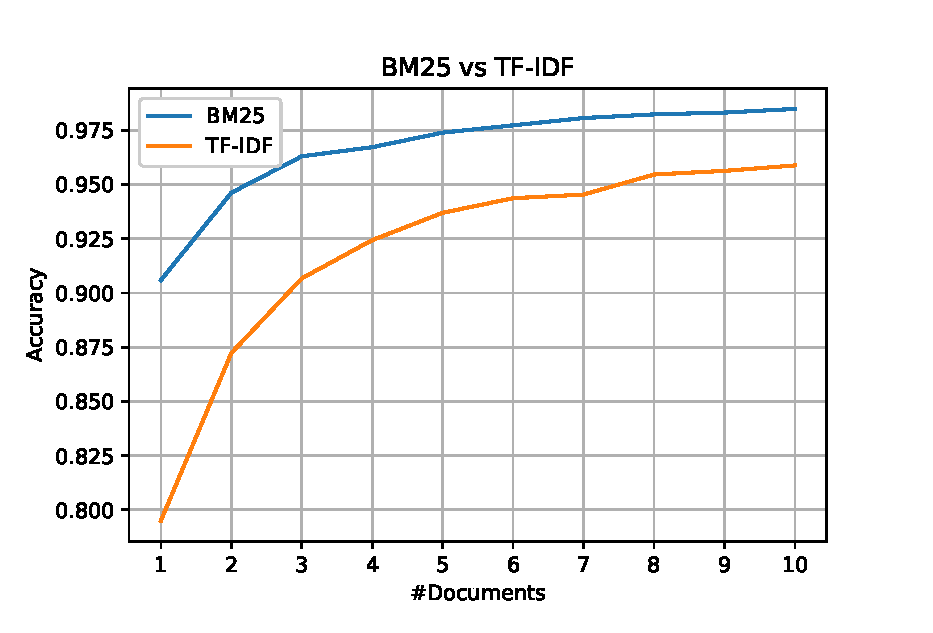
\includegraphics[width=\linewidth]{figures/chapter6/test.eps}
  \caption{Ακρίβεια \emph{BM25 Retriever} και \emph{TF-IDF Retriever} στο \emph{SQuAD} σύνολο δεδομένων}
  \label{bm25-acc}
\end{figure}

% \begin{figure}[htb]
%   \centering
%   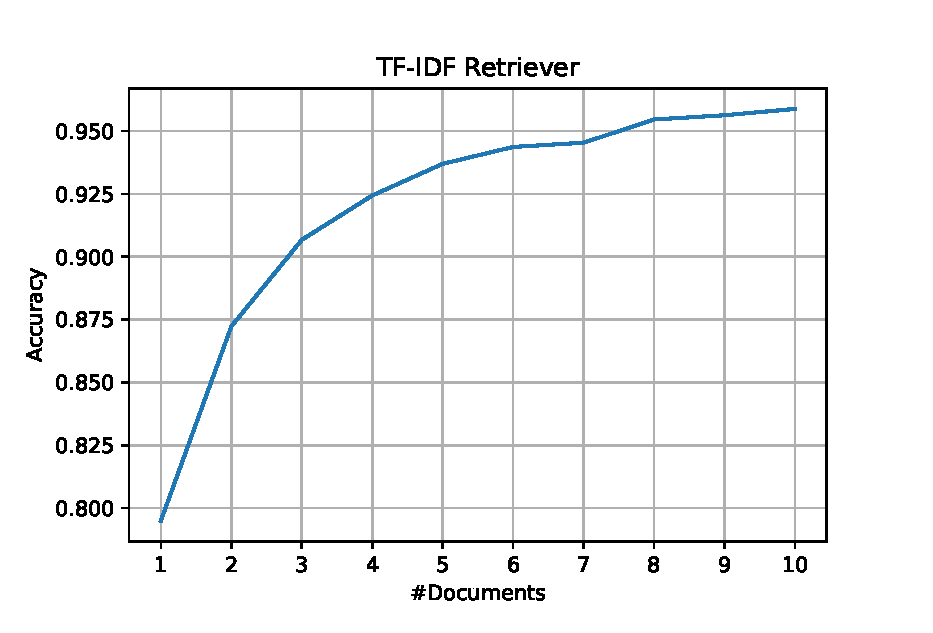
\includegraphics[width=\linewidth]{figures/chapter6/tf-idf-acc.eps}
%   \caption{Ακρίβεια \emph{TF-IDF Retriever} στο \emph{SQuAD} σύνολο δεδομένων}
%   \label{tfidf-acc}
% \end{figure}

\section{\emph{Reader}}
\label{sec:reader_exp}
Ο \emph{Reader} αποτελεί έναν από τους σημαντικότερους κόμβους του συστήματος. Τα πειράματα που πραγματοποιήθηκαν μελέτησαν την απόδοση διάφορων μοντέλων στην εύρεση απάντησης σε κείμενο το οποίο περιείχε τη σωστή απάντηση. Επίσης, μελετήθηκαν διάφορα μήκη εισόδων στα μοντέλα (\emph{max\_seq\_len}) και διαφορετικό βήμα κινούμενου παραθύρου (\emph{doc\_stride}). Από τους πίνακες \ref{tab:reader_scores1}, \ref{tab:reader_scores2} φαίνεται ότι το μοντέλο με τη μεγαλύτερη απόδοση είναι το \emph{xlm-roberta-large-squad2}\footnote{\url{https://huggingface.co/deepset/xlm-roberta-large-squad2}} από την \emph{deepset} το οποίο είναι εκπαιδευμένο στο \emph{SQuAD2}\footnote{\url{https://rajpurkar.github.io/SQuAD-explorer/explore/v2.0/dev/}} και χρησιμοποιείται με τη μέθοδο \emph{zero-shot}, καθώς δεν είναι εκπαιδευμένο στα ελληνικά. Επιπλέον, τα δύο ελληνικά μοντέλα \emph{squad\_bert\_el}\footnote{\url{https://huggingface.co/Danastos/squad_bert_el}} και \emph{qacombination\_bert\_el}\footnote{\url{https://huggingface.co/Danastos/qacombination_bert_el}} έχουν παρόμοια απόδοση. Οι παράμετροι \emph{max\_seq\_len} και \emph{doc\_stride} επιλέχθηκαν με τις τιμές $256$ και $128$ αντίστοιχα, καθώς η απόδοση του με μεγαλύτερες τιμές παρουσίασε ελάχιστη βελτίωση. Ταυτόχρονα αξίζει να σημειωθεί ότι τα ελληνικά μοντέλα προβλέπουν σε μικρότερο χρόνο από ότι το \emph{xlm-roberta-large-squad2}, το οποίο ήταν αναμενόμενο γνωρίζοντας ότι το μέγεθος του τελευταίου. Το μοντέλο που χρησιμοποιήθηκε στη παρούσα υλοποίηση ήταν \emph{xlm-roberta-large-squad2}\footnote{Το μοντέλο \emph{xlm-roberta-large-squad2} έχει max\_seq\_len 256, επομένως στο πείραμα με τα 512 το παράθυρο δεν επικαλύπτει τη προηγούμενη με την επόμενη είσοδο}, καθώς η ακρίβεια του μοντέλου είναι κύριας σημασίας για το σύστημα.

\begin{table}[!htb]
    \captionsetup{justification=centering}
    \begin{center}
        \caption{\emph{Accuracy} και \emph{$F_1$ Score} των μοντέλων \emph{Reader} με \emph{max\_input\_length}=$256$ και \emph{doc\_stride=$128$}}
        \begin{tabular}{ | c | c | c | }
            \hline
            \rowcolor{Gray}
            Μοντέλο & \textbf{\emph{$EM$}} & \textbf{\emph{$F_1 Score$}}\\
            xlm-roberta-large-squad2 & $55.7$ & $75.8$\\
            squad\_bert\_el & $57.1$ & $74.9$\\
            qacombination\_bert\_el & $55.6$ & $74.3$\\
            newsqa\_bert\_el & $39.2$ & $58.8$\\
            nq\_bert\_el & $38.5$ & $57.5$\\
            triviaqa\_bert\_el & $27.9$ & $40.9$\\
            \hline
        \end{tabular}
        \label{tab:reader_scores1}
    \end{center}
\end{table}

\begin{table}[H]
    \captionsetup{justification=centering}
    \begin{center}
        \caption{\emph{Accuracy} και \emph{$F_1$ Score} των μοντέλων \emph{Reader} με \emph{max\_input\_length}=$512$ και \emph{doc\_stride=$256$}}
        \begin{tabular}{ | c | c | c | }
            \hline
            \rowcolor{Gray}
            Μοντέλο & \textbf{\emph{$EM$}} & \textbf{\emph{$F_1 Score$}}\\
            xlm-roberta-large-squad2 & $56.4$ & $76.8$\\
            squad\_bert\_el & $57.1$ & $74.8$\\
            qacombination\_bert\_el & $55.6$ & $74.1$\\
            newsqa\_bert\_el & $39.2$ & $58.6$\\
            nq\_bert\_el & $38.5$ & $57.7$\\
            triviaqa\_bert\_el & $27.5$ & $40.7$\\
            \hline
        \end{tabular}
        \label{tab:reader_scores2}
    \end{center}
\end{table}